% !TeX root = ../main.tex

\chapter{Background}\label{chapter:background}

	%In this chapter, \dots

	%\section{Math} \label{sec:full_grids}
	
		%Math:
		%\begin{align}
			%\Phi(x) = \max(1 - \abs{x}, 0)
		%\end{align}
		
	 %\subsection{Example Figure} \label{sec:back_nodal_hierarchical_basis}
		
		%\begin{figure}[htbp]
			%\centering
			%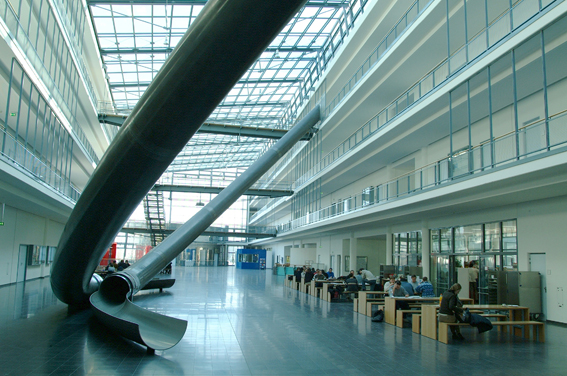
\includegraphics[width=0.5\textwidth]{figures/tum.jpg}
			%\caption{Example picture that was taken from an external source \takenFrom{asc_notes}.}
			%\label{fig:nodalBasis}
		%\end{figure}
		
		%References on figures work like this: blblablabla (see \refFigure{fig:nodalBasis}). If you used external knowledge for a paragraph, use the cite command at the very end of a sentence but right before the full stop \cite{ba_molzer}.
		
		%If you use an $l$ for math symbols, use $\ell$ instead for better readability.
		
	\section{Priorisieren von Benutzeroberflächen}
	- Prioritätsgruppen
	- Umsetzung in 2D
		
	\section{Positionierung in 2D}
	- Fenstergebunden WIMP
	- Menüs / Fenster
	- Bildschirmränder
		
	\section{Positionierung in 3D (VR/AR auch ohne)}
	- 3D Programm: UI in Welt platziert
	- Üblich Hände und Kopf 
	- Beispiele!
	- dreidimensionale Benutzeroberflächen